\section{Marco teórico}

\subsection{Transformador Monofásico}
El transformador monofásico es una máquina eléctrica sin elementos móviles que permite transferir energía entre circuitos mediante el fenómeno de la inducción mutua, sustentado en las leyes de Faraday y Lenz. Diseñado para trabajar con señales alternas sinusoidales de fase única, consta conceptualmente de dos devanados uno primario y otro secundario enlazados mediante un núcleo de material ferromagnético de chapas laminadas. Bajo un enfoque ideal en el que se omiten las pérdidas internas, este equipo ajusta las magnitudes de voltaje y corriente en el sistema conservando invariable la potencia aparente, todo ello operando con un alto rendimiento energético. 

\begin{figure}[H]
    \centering
    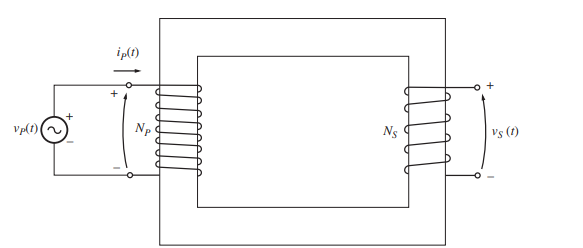
\includegraphics[width=0.7\linewidth]{imagenes/1.transformador monofasico.png}
    \caption{Dibujo de un transformador monofasico} 
\end{figure}

\subsection{Devanado Primario y Secundario}

En un transformador monofásico, los devanados primario y secundario son los dos circuitos inductivos de hilo conductor (generalmente cobre o aluminio) enrollados alrededor del núcleo magnético común, encargados de realizar la conversión de energía eléctrica a magnética y viceversa:

\begin{itemize}
    \item \textbf{Devanado Primario:} Es el arrollamiento de entrada conectado directamente a la fuente de alimentación de corriente alterna. Su función principal es recibir la energía eléctrica e magnetizar el núcleo ferromagnético, generando un flujo magnético variable en el tiempo que circula a través del circuito magnético.
    
    \item \textbf{Devanado Secundario:} Es el arrollamiento de salida conectado a la carga eléctrica. Al ser atravesado por el flujo magnético alterno generado por el primario, en sus terminales se induce una fuerza electromotriz (tensión inducida) según la ley de Faraday, entregando así la energía convertida a los equipos o al sistema receptor.
\end{itemize}

La relación entre el número de espiras del primario ($N_1$) y del secundario ($N_2$) define la relación de transformación ($a$), dada por:

\begin{equation}
    a = \frac{N_1}{N_2}
\end{equation}

Esta proporción determina si el dispositivo opera como un transformador elevador ($N_2 > N_1$) o reductor ($N_2 < N_1$) de tensión.

\subsection{Transformador real}
A diferencia del modelo teórico, el transformador real considera los efectos resistivos y magnéticos derivados del comportamiento físico de los componentes. La presencia de la resistencia propia de los conductores en el devanado primario y secundario genera disipación de potencia en forma de calor por efecto Joule. Asimismo, la dispersión del flujo magnético origina reactancias que provocan variaciones e impedancias adicionales en el voltaje de salida al operar bajo carga. Por otro lado, la no idealidad del núcleo ferromagnético requiere una corriente de magnetización para sostener el flujo mutuo e induce pérdidas internas compuestas por la energía disipada en los ciclos de histéresis y la circulación de corrientes parásitas o de Foucault.

\begin{figure}[H]
    \centering
    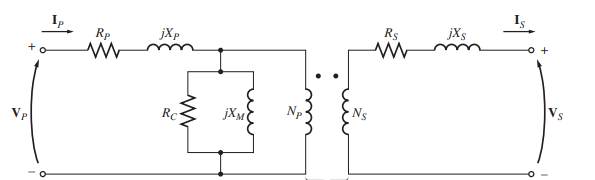
\includegraphics[width=0.85\linewidth]{imagenes/transformador real .png}
    \caption{Modelo del Transformador Real}
\end{figure}

\subsection{Transformador referido al primario}
Para simplificar la resolución del circuito equivalente reflejando toda la red a un único nivel de tensión, se aplica la técnica de referenciación hacia el primario. Mediante la relación de transformación $a = N_1/N_2$, la impedancia, el voltaje y la corriente del secundario se escalan hacia la entrada, eliminando la discontinuidad galvánica del transformador ideal intermedio sin alterar las condiciones energéticas del sistema.

\begin{figure}[H]
    \centering
    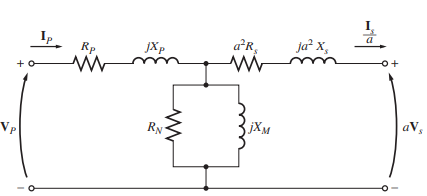
\includegraphics[width=0.85\linewidth]{imagenes/referido al primario.png}
    \caption{Modelo del transformador referido a su nivel de voltaje
primario}
\end{figure}

\subsection{Transformador referido al secundario}
El acoplamiento del circuito al lado secundario consiste en proyectar las magnitudes eléctricas del devanado primario hacia el devanado de menor o mayor voltaje según sea el caso de carga. Aplicando la relación de vueltas de manera inversa, las impedancias del primario se dividen entre $a^2$, preservando la equivalencia matemática en los balances de potencia activa y reactiva del conjunto.

\begin{figure}[H]
    \centering
    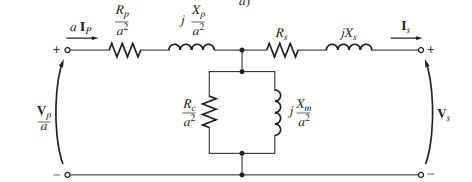
\includegraphics[width=0.85\linewidth]{imagenes/referido al secuendario.png}
    \caption{Modelo del transformador referido a su nivel de voltaje
secundario}
\end{figure}

\subsection{ Comportamiento Bajo Cargas Lineales}

Cuando el transformador alimenta cargas lineales (resistencias, inductores o condensadores puros), las formas de onda de tensión y corriente permanecen senoidales.
\begin{itemize}
    \item En \textbf{cargas resistivas}, la corriente y la tensión están en fase, por lo que la potencia activa ($P$) coincide con la potencia aparente ($S$), al tener un factor de potencia unitario.
    \item Las pérdidas internas del transformador provocan que, al cargar el equipo, la tensión de salida sea siempre menor que la tensión en vacío.
\end{itemize}

\subsection{ Comportamiento Bajo Cargas No Lineales}

Las cargas no lineales, como los rectificadores, absorben corrientes cuya forma de onda no es proporcional a la tensión aplicada. Esto genera efectos significativos:
\begin{itemize}
    \item \textbf{Corrientes Armónicas:} El rectificador de onda completa es un generador característico de armónicos, que son componentes de corriente con frecuencias múltiples de la fundamental.
    \item \textbf{Distorsión de Formas de Onda:} Estos armónicos provocan que la corriente se distorsione, afectando tanto al lado primario como al secundario del transformador.
    \item \textbf{Aumento de Pérdidas:} La circulación de armónicos eleva las pérdidas en el cobre debido al efecto Joule y al efecto piel, además de aumentar marginalmente las pérdidas en el núcleo.
    \item \textbf{Factor de Potencia y Potencias:} Al existir potencia de distorsión ($D$), la potencia aparente ($S$) resulta mayor que la activa ($P$), cumpliendo que $S^2 = P^2 + Q^2 + D^2$. Los instrumentos de medida deben ser del tipo RMS para capturar correctamente estos valores.
    \item \textbf{Desclasificación (Derating):} Ante el riesgo de sobrecalentamiento por armónicos, es necesario operar el transformador por debajo de su capacidad nominal (derating) o utilizar transformadores con factor K, diseñados específicamente para manejar este tipo de carga.
\end{itemize}

\subsection{Regulación de tensión}
La regulación de tensión ($\text{Reg\%}$) se define como el parámetro numérico que cuantifica la variación porcentual en la magnitud del voltaje en las terminales del secundario de un transformador cuando este pasa de operar en una condición de vacío (sin carga) a su estado de plena carga nominal. Este indicador mide la capacidad del dispositivo para mantener la estabilidad del nivel de tensión entregado a los usuarios frente a fluctuaciones en la demanda de la carga.

Matemáticamente, la regulación de tensión se expresa como:

\begin{equation}
    \text{Reg\%} = \frac{|V_{2,\text{vacío}}| - |V_{2,\text{carga}}|}{|V_{2,\text{carga}}|} \times 100\%
\end{equation}

donde:
\begin{itemize}
    \item $|V_{2,\text{vacío}}|$ es la magnitud de la tensión en el devanado secundario cuando la corriente de salida es nula ($I_2 = 0$).
    \item $|V_{2,\text{carga}}|$ es la magnitud de la tensión medida en las terminales del secundario cuando circula la corriente nominal de carga.
\end{itemize}

\paragraph{Criterios de interpretación:}
\begin{itemize}
    \item \textbf{Modelo Ideal ($\text{Reg\%} = 0\%$):} El voltaje en los bornes permanece perfectamente constante independientemente de la corriente demandada.
    \item \textbf{Cargas Resistivas e Inductivas ($\text{Reg\%} > 0$):} El voltaje bajo carga disminuye respecto al voltaje en vacío a causa de las caídas de tensión internas en la impedancia equivalente ($I \cdot Z$).
    \item \textbf{Cargas Capacitivas ($\text{Reg\%} < 0$):} Ocurre un fenómeno de elevación de tensión donde el voltaje en carga supera al voltaje en vacío debido al desfase de la corriente en adelanto.
\end{itemize}